\section{Logische Gatter}

\textbf{Realisierungsaufwand:} Anzahl Transistoren ist ein m"ogliches Mass f"ur die Komplexit"at (Marketing). In der Technik spricht man von Gatter"aquivalent: 1 Gatter"aquivalent entspricht 4 Transistoren. \\ 
\textbf{Anzahl Schaltfunktionen:} $F= {2^2}^n$, n: Anzahl Eing"ange

\subsection{Verhalten logischer Gatter}
	\begin{minipage}[c]{8 cm}
		\subsubsection{St"orabstand}
			High-Pegel: $ U_{nH} = U_{aHmin} - U_{eHmin} $\\
			Low-Pegel: $ U_{nL} = U_{eLmax} - U_{aLmax} $\\	
			\newline
			\newline
			\newline			
	\end{minipage}	
	\begin{minipage}[c]{6 cm}
		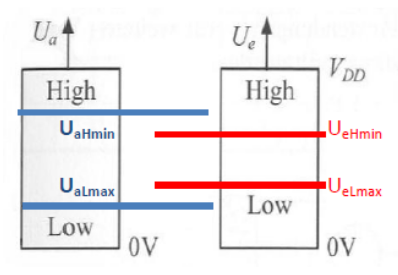
\includegraphics[width=0.9\textwidth]{pics/Pegelbereiche_Stoerabstand}
	\end{minipage}

	\subsubsection{Propagation delay Time Anstiegs-/Abstiegszeit}
		\begin{minipage}[c]{8 cm}
			Zeit zwischen 50\% von $V_{max}$ am Eingang und 50\% von $V_{max}$ am Ausgang.\\
			\newline
			$t_{pd}=\frac{t_{pLH}+t{pHL}}{2}$\\
		\end{minipage}	
		\begin{minipage}[c]{10 cm}
			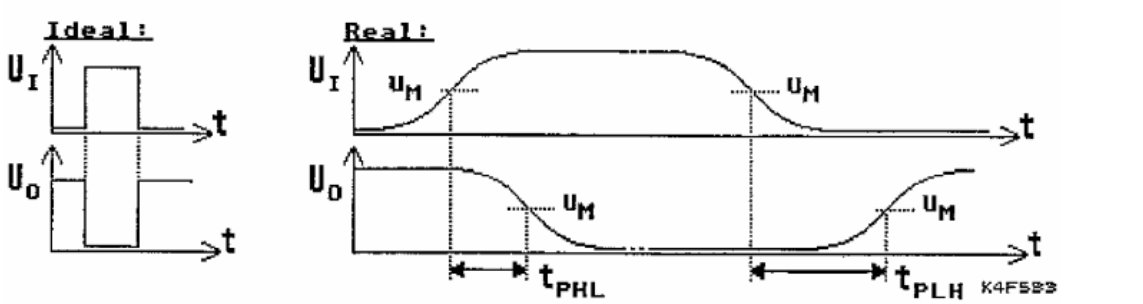
\includegraphics[width=0.9\textwidth]{pics/delay}
		\end{minipage}	
		
	\subsubsection{Transition delay Time (Verz"ogerungszeit)}
		Zeit zwischen 10\% und 90\% von $V_{max}$.\\
		$t_{tLH}$: Transition time low to high.\\
		$t_{tHL}$: Transition time high to low.\\
		
\subsection{Hazards}
	\begin{minipage}[c]{9 cm}
		\subsubsection{Statischer Hazard}
			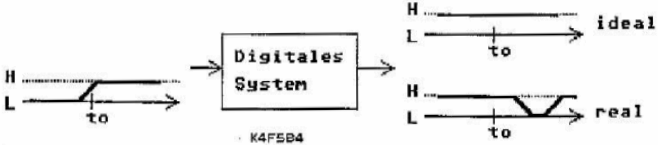
\includegraphics[width=1\textwidth]{pics/hazardstatisch}
			Der Funktionswert eines kombinatorischen Systems "andert kurzzeitig seinen Pegel, wenn eine Eingangsvariable den Pegel "andert, obschon von der logischen Funktion keine "Anderung gegeben ist.
	\end{minipage}
	\begin{minipage}[c]{9 cm}	
		\subsubsection{Dynamischer Hazard}
			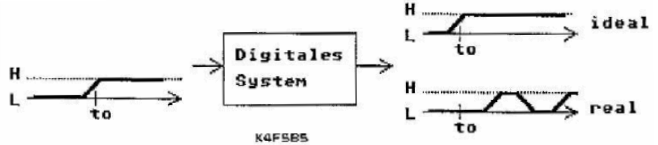
\includegraphics[width=1\textwidth]{pics/hazarddynamisch}
			Der Funktionswert eines kombinatorischen Systems "andert mehrmals kurzzeitig seinen Pegel, wenn eine Eingangsvariable den Pegel "andert, obschon von der logischen Funktion her nur eine einzige "Anderung erfolgen sollte.
	\end{minipage}
	
\begin{sidewaystable}
	\subsection{Aufbau logischer Gatter}
		\begin{tabular}{|c|c|c|c|c|c|c|c|c|}
			\hline
				Funktion & Buffer & NOT & AND & NAND & OR & NOR & EXOR & XNOR\\
				& & Nicht & Und & Nicht Und & Oder & Nicht Oder & Exklusiv Oder & Nicht Ex. Oder\\
				& & Inverter & Konjunktion & & Disjunktion & & Antivalenz & "Aquivalenz \\
			\hline
				Formel & a & $ \overline a $ & $ a * b $ & $ \overline{a * b} $ & $ a + b $ & $ \overline{a + b} $ & $ a \oplus b $ & $ \overline{a \oplus b} $\\
				& a & $ \overline a $ & $ a \wedge b $ & $ \overline{a \wedge b} $ & $ a \vee b $ & $ \overline{a \vee b} $ & $ a \$ b $ & $ \overline{a \$ b} $ \\
			\hline
				Symbol & & & & & & & &\\
				& 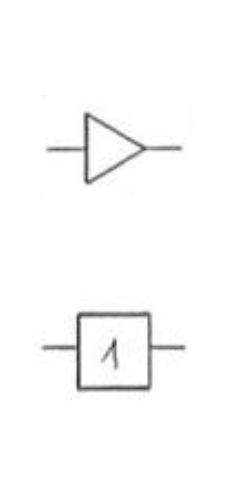
\includegraphics[width=0.08\textwidth]{pics/gates_symbol/buffer} & 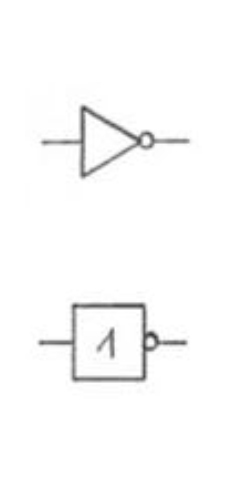
\includegraphics[width=0.08\textwidth]{pics/gates_symbol/not} & 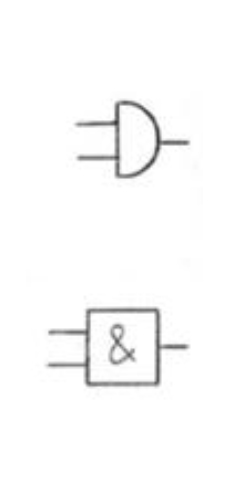
\includegraphics[width=0.08\textwidth]{pics/gates_symbol/and} & 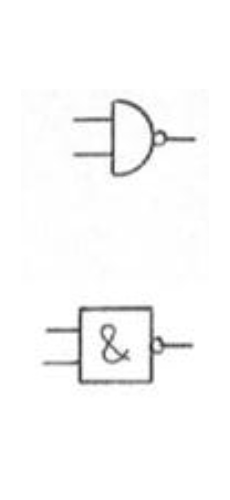
\includegraphics[width=0.08\textwidth]{pics/gates_symbol/nand} & 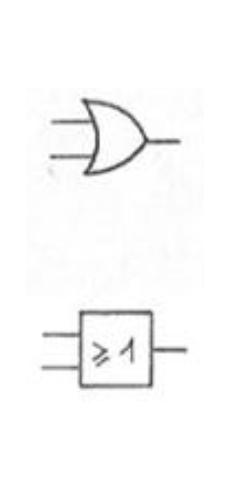
\includegraphics[width=0.08\textwidth]{pics/gates_symbol/or} & 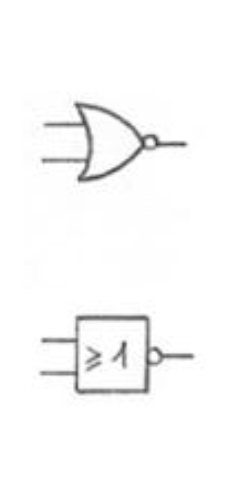
\includegraphics[width=0.08\textwidth]{pics/gates_symbol/nor} & 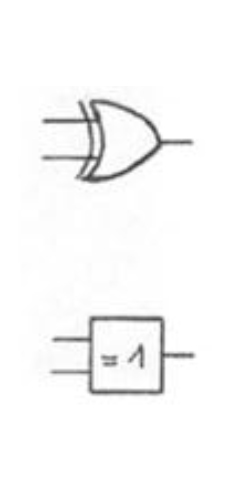
\includegraphics[width=0.08\textwidth]{pics/gates_symbol/exor} & 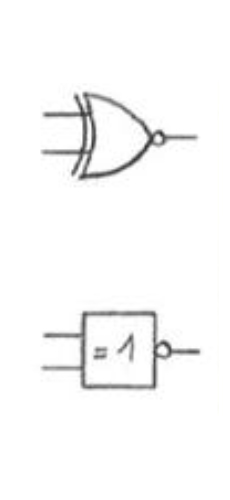
\includegraphics[width=0.08\textwidth]{pics/gates_symbol/xnor} \\
			\hline
				WHT & & & & & & & &\\
				(0,0) & 0 & 1 & 0 & 1 & 0 & 1 & 0 & 1\\
				(0,1) &   &   & 0 & 1 & 1 & 0 & 1 & 0\\
				(1,0) & 1 & 0 & 0 & 1 & 1 & 0 & 1 & 0\\
				(1,1) &   &   & 1 & 0 & 1 & 0 & 0 & 1\\
			\hline
				& 
				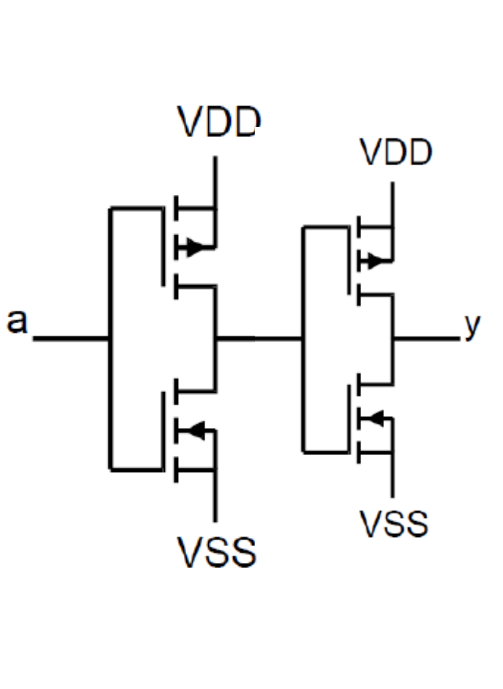
\includegraphics[width=0.1\textwidth]{pics/gates_schematic/buffer} & 
				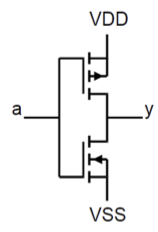
\includegraphics[width=0.08\textwidth]{pics/gates_schematic/inverter} & 
				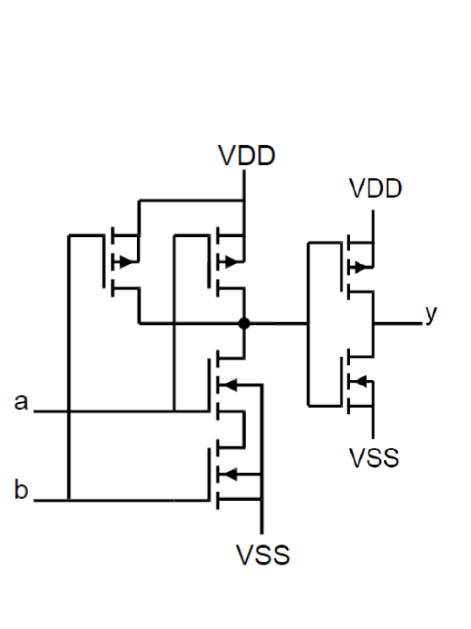
\includegraphics[width=0.1\textwidth]{pics/gates_schematic/and} &
				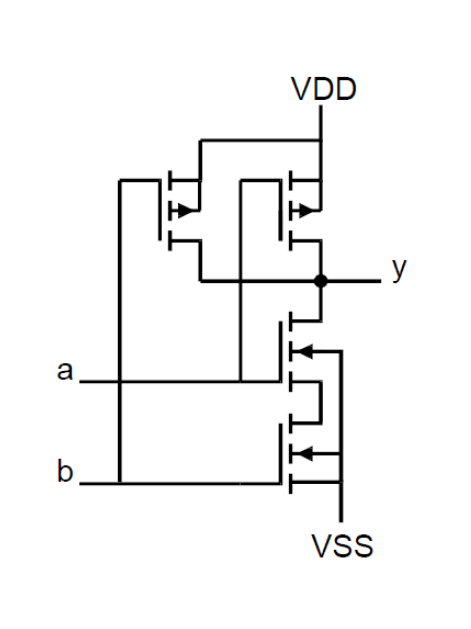
\includegraphics[width=0.1\textwidth]{pics/gates_schematic/nand} &
				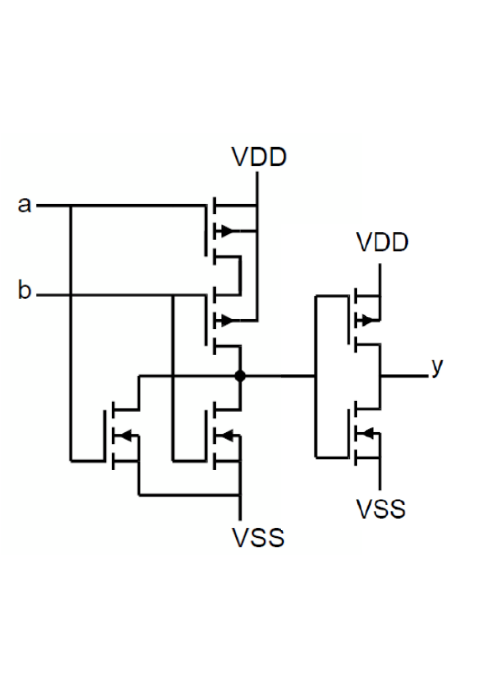
\includegraphics[width=0.1\textwidth]{pics/gates_schematic/or} &
				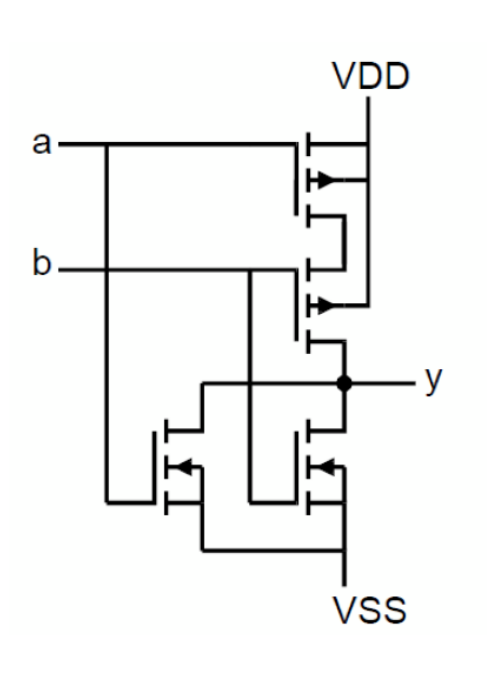
\includegraphics[width=0.1\textwidth]{pics/gates_schematic/nor} & 
				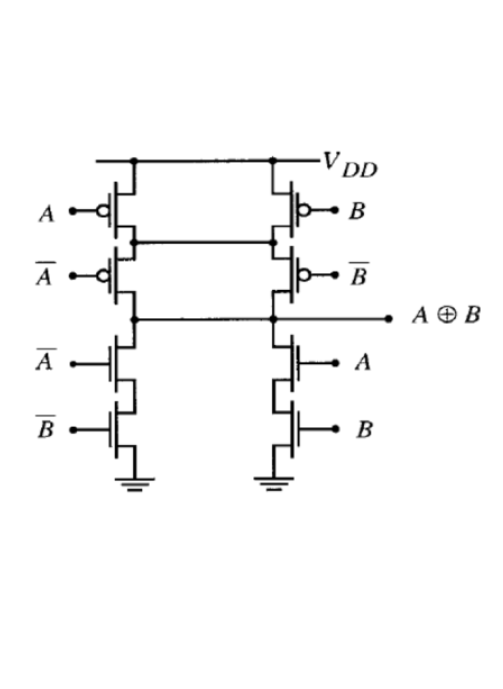
\includegraphics[width=0.1\textwidth]{pics/gates_schematic/xor} & 
				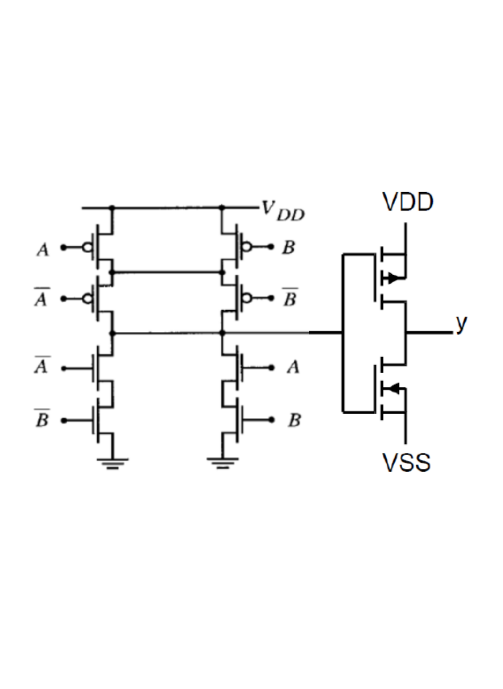
\includegraphics[width=0.1\textwidth]{pics/gates_schematic/xnor} \\
			\hline
				Trans & 4 & 2 & 6 & 4 & 6 & 4 & 8 & 10\\
			\hline
		\end{tabular}
\end{sidewaystable}